%% Template.tex; Solar Physics
%% 
\documentclass[namedreferences]{SolarPhysics}
%
% spr-sola-addons available options:
%  natbib        -- For citations: redefine \cite commands
%  solaenum      -- makes enumerated list with italics-roman numerals and a single right-bracket
%  linksfromyear -- loads a natbib and puts a link on a year citation (hyperref must be loaded)
%  optionalrh    -- for optional running title/author
%
%\usepackage[optionalrh,solaenum]{spr-sola-addons} % For Solar Physics 
%\usepackage{epsfig}                     % For eps figures, old commands
\usepackage{graphicx}                    % For eps figures, newer & more powerfull
%\usepackage{courier}                    % Change the \texttt command to courier style
%\usepackage{amssymb}                    % useful mathematical symbols
\usepackage{color}                       % For color text: \color command
\usepackage{url}                         % For breaking URLs easily trough lines
\def\UrlFont{\sf}                        % define the fonts for the URLs

%% Local definitions
%% please place your own definitions here and don't use \def but
%% \newcommand{}{} or 
%% \renewcommand{}{} if it is already defined in LaTeX

%I'm adding these:
\usepackage[optionalrh,natbib]{spr-sola-addons}
\newcommand{\solphys}{{\it Solar Physics}}
\newcommand{\aap}{    {\it Astronomy \& Astrophysics}}
\newcommand{\aaps}{   {\it Astronomy \& Astrophysics Supplemental}}
\newcommand{\apj}{    {\it Astrophysical Journal}}
\newcommand{\apjl}{    {\it Astrophysical Journal Letters}}
\newcommand{\jgr}{    {\it Journal of Geophysical Research}}
\newcommand{\aapr}{    {\it Astronomy \& Astrophysics Review}}
\newcommand{\grl}{    {\it Geophysical Research Letters}}



%%%%%%%%%%%%%%%%%%%%%%%%%%%%%%%%%%%%%%%%%%%%%%%%%%%%%%%%%%%%%%%%%%
\begin{document}

\begin{article}

%%%%%%%%%%%%%%%%%%%%%%%%%%%%%%%%%%%%%%%%%%%%%%%%%%%
%% Sections
%
% \section{}%\label{s:?} 

\section{Automatic Detection \& Tracking of CMEs}

\subsection{Normalising Radial Graded Filter}
\label{sect_nrgf}

This will introduce the model as a test for the NRGF

\subsection{Dynamic / Quiescent Separation Technique}
\label{sect_separation}

... and more model discussion to show the efficacy of the methods.

\subsection{Multiscale Filtering}

Following directly from the processing steps described above, namely the NRGF and quiescent background separation, a method of multiscale filtering may be employed to detect and track CME structure in the images. The fundamental idea behind multiscale analysis is to highlight details apparent on different scales within the data. An example of this is the suppression of noise in images, which tends to occur only on the smallest scales. Wavelets, as a multiscale tool, have benefits over other traditional methods, such as Fourier transforms, because they are localised in space and are easily dilated and translated in order to operate on multiple scales. The fundamental equation is given by:
\begin{equation}
\psi_{a,b}(t)\,=\, \frac{1}{\sqrt{b}} \, \psi (\frac{t-a}{b})
\end{equation}
where $a$ and $b$ represent the shifting (translation) and scaling (dilation) of the mother wavelet $\psi$ which can take several forms depending on the required use. Details on the application of high and low pass filters on multiple scales is outlined in \citet{2008SoPh..248..457Y} and shown by \citet{2009A&A...495..325B, 2010NatCo...1E..74B} to be effective for studying CMEs in coronagraph data. Thus we follow the same filtering techniques here, but exploit the derived information to such an extent that the CME structure may be automatically detected and characterized in a series of images. The multiscale decomposition in 2D is performed through the use of low and high pass filters; using a discrete approximation of a Gaussian, $\theta$, and its derivative, $\psi$, respectively. Since $\theta(x,y)$ is separable, i.e., $\theta(x,y)=\theta(x)\theta(y)$, we can write the wavelets as the first derivative of the smoothing function:
\begin{eqnarray}
\psi_{x}^{s}(x,y)\,&=\, s^{-2} \frac{\partial \theta(s^{-1}x)}{\partial x}\theta(s^{-1}y) \\
\psi_{y}^{s}(x,y)\,&=\, s^{-2} \theta(s^{-1}x)\frac{\partial \theta(s^{-1}y)}{\partial y}
\end{eqnarray}
where $s$ is the dyadic scale factor such that $s=2^j$ for $j=1,2,3,...,J~\in~\mathbb{N}$. Successive convolutions of an image with the filters produce the scales of decomposition, with the high-pass filtering providing the wavelet transform of image $I(x,y)$ in each direction:
\begin{eqnarray}
W_{x}^{s}I \,&\equiv\, W_{x}^s I(x,y)\,=\,\psi_{x}^s (x,y)*I(x,y) \\
W_{y}^{s}I \,&\equiv\, W_{y}^s I(x,y)\,=\,\psi_{y}^s (x,y)*I(x,y)
\end{eqnarray}
Akin to a Canny edge detector, these horizontal and vertical wavelet coefficients are combined to form the gradient space, $\Gamma^s(x,y)$, for each scale: 
\begin{equation}
\Gamma^s (x,y)\, = \,\left[W_{x}^s I,~W_{y}^s I \right]
\end{equation}
The gradient information has an angular component $\alpha$ and a magnitude (edge strength) $M$:
\begin{eqnarray}
\alpha^s(x,y) \, &= \, tan^{-1}\left( W_{y}^s I~/~W_{x}^s I \right) \\
M^s(x,y) \, &= \, \sqrt{ ( W_{x}^s I ) ^2 + ( W_{y}^s I ) ^2 }
\end{eqnarray}
Figure~\ref{figure_model8} shows the resulting magnitude (panels $a$ and $b$) and angular information (panels $c$ and $d$) for a particular scale ($s=2^{4}$) of the decomposition applied to the model CME images. This information is then used to generate a CME detection mask for each image.


\begin{figure}[!p*]
\centerline{\includegraphics[scale=1.2, clip=true, trim=0 330 260 10]{images/figure_model8.pdf}}
\caption{A snapshot of the algorithms applied to the model CMEs A and B. Panels ($a$) and ($b$) show the magnitude information (edge strength), and ($c$) and ($d$) show the angular information, at a particular scale of the multiscale decomposition. Panels ($e$) and ($f$) show the resulting CME detection masks following the scoring system. Panels ($g$) and ($h$) show the final CME structure detection overlaid in yellow on the model C2 and C3 images. The edges were determined using a pixel-chaining algorithm on the magnitude and angular information of the multiscale decomposition.}
\label{figure_model8}
\end{figure}

\subsection{CME Detection Mask}

The scales upon which the multiscale filtering best resolves the CME have dyadic scale factors of $s=2^{2},\,2^{3},\,2^{4},\,2^{5}$. The discarded finer scales detail mostly the noise, and the coarser scales overly smooth the CME signal. At each of these four scales, the corresponding magnitude $M$ is thresholded at 1.5\,$\sigma$ ($\sigma$ is standard deviation) above the mean intensity level, resulting from inspection of the method applied to a sample of ten different CMEs. This results in regions-of-interest (ROIs) on each image that may be tested as possible CMEs since they meet the criteria that they are bright features, consequently having stronger edges. To make the 1.5\,$\sigma$ threshold somewhat softer, the initial ROIs are removed and the threshold reapplied at 1.5\,$\sigma$ of the remaining image data to obtain new ROIs. The difference between the new and original ROIs is quantified by subtracting the number of pixels in each, and the intensity threshold reapplied if the subsequent ROI pixel difference is greater than the preceding difference. If the quantified difference decreases, signaling that nothing more can be gained by continuing to soften the threshold on the magnitude image, the threshold is fixed and used to determine the final ROIs. The angular information is then determined for each of these ROIs, since a curvilinear feature will have a wider distribution of angles than a radial feature or a point source in the decomposition. The angular distributions of the individual ROIs are folded from ranges 0\,--\,360$^{\circ}$ to 0\,--\,180$^{\circ}$ due to their symmetry, and the distribution is normalised to unity. The median value of the distribution across each ROI is then thresholded as a measure for scoring the validity of the detection in order to build up a detection mask of the image:
\begin{enumerate}
\item if the median angular value is $>$\,20\,\% of the distribution peak then the region is deemed a CME and assigned a score of 3 (the pixels in that ROI are given the value 3);
\item if it is $>$\,10\,\% the score is 2 (potential CME structure);
\item if it is $>$\,5\,\% the score is 1 (weak CME structure or part thereof).
\end{enumerate}
Figure~\ref{figure_model8}$e$ and $d$ show the resulting CME detection mask built up in this manner for the model CME images. Immediately it is possible to remove the areas of the mask that do not additively achieve a strong enough detection. So, again by inspection across a test sample of ten events, the masks are thresholded at a level $>$\,3 since only the regions that achieve a sufficient score to be classified as a CME detection are included.

Now that a CME detection has been established, its structure is defined by the edges determined in the pixel-chaining algorithm applied at the scale of $s=2^{4}$ since that scale most consistently exhibits the highest signal-to-noise ratio for the ten sample events. Since the CME detection mask was built with four scales, it is now eroded by a factor of 8 pixels to account somewhat for the amount of smoothing involved in the coarser of the scales used, recalling that the low scoring regions of the detection mask have already been removed. This limits the detection mask to more appropriately lie over the true CME edges and reduce any overlap with the surrounding image noise. Figure~\ref{figure_model8}$g$ and $h$ show the resultant CME structure detections overlaid on the original model images. While there is still an element of noise in the detections, clear structure along the magnetic field topology of the erupting CME plasma is defined - and automatically so.


\section{Structure \& Kinematics of CMEs}

\begin{figure}[!t]
\centerline{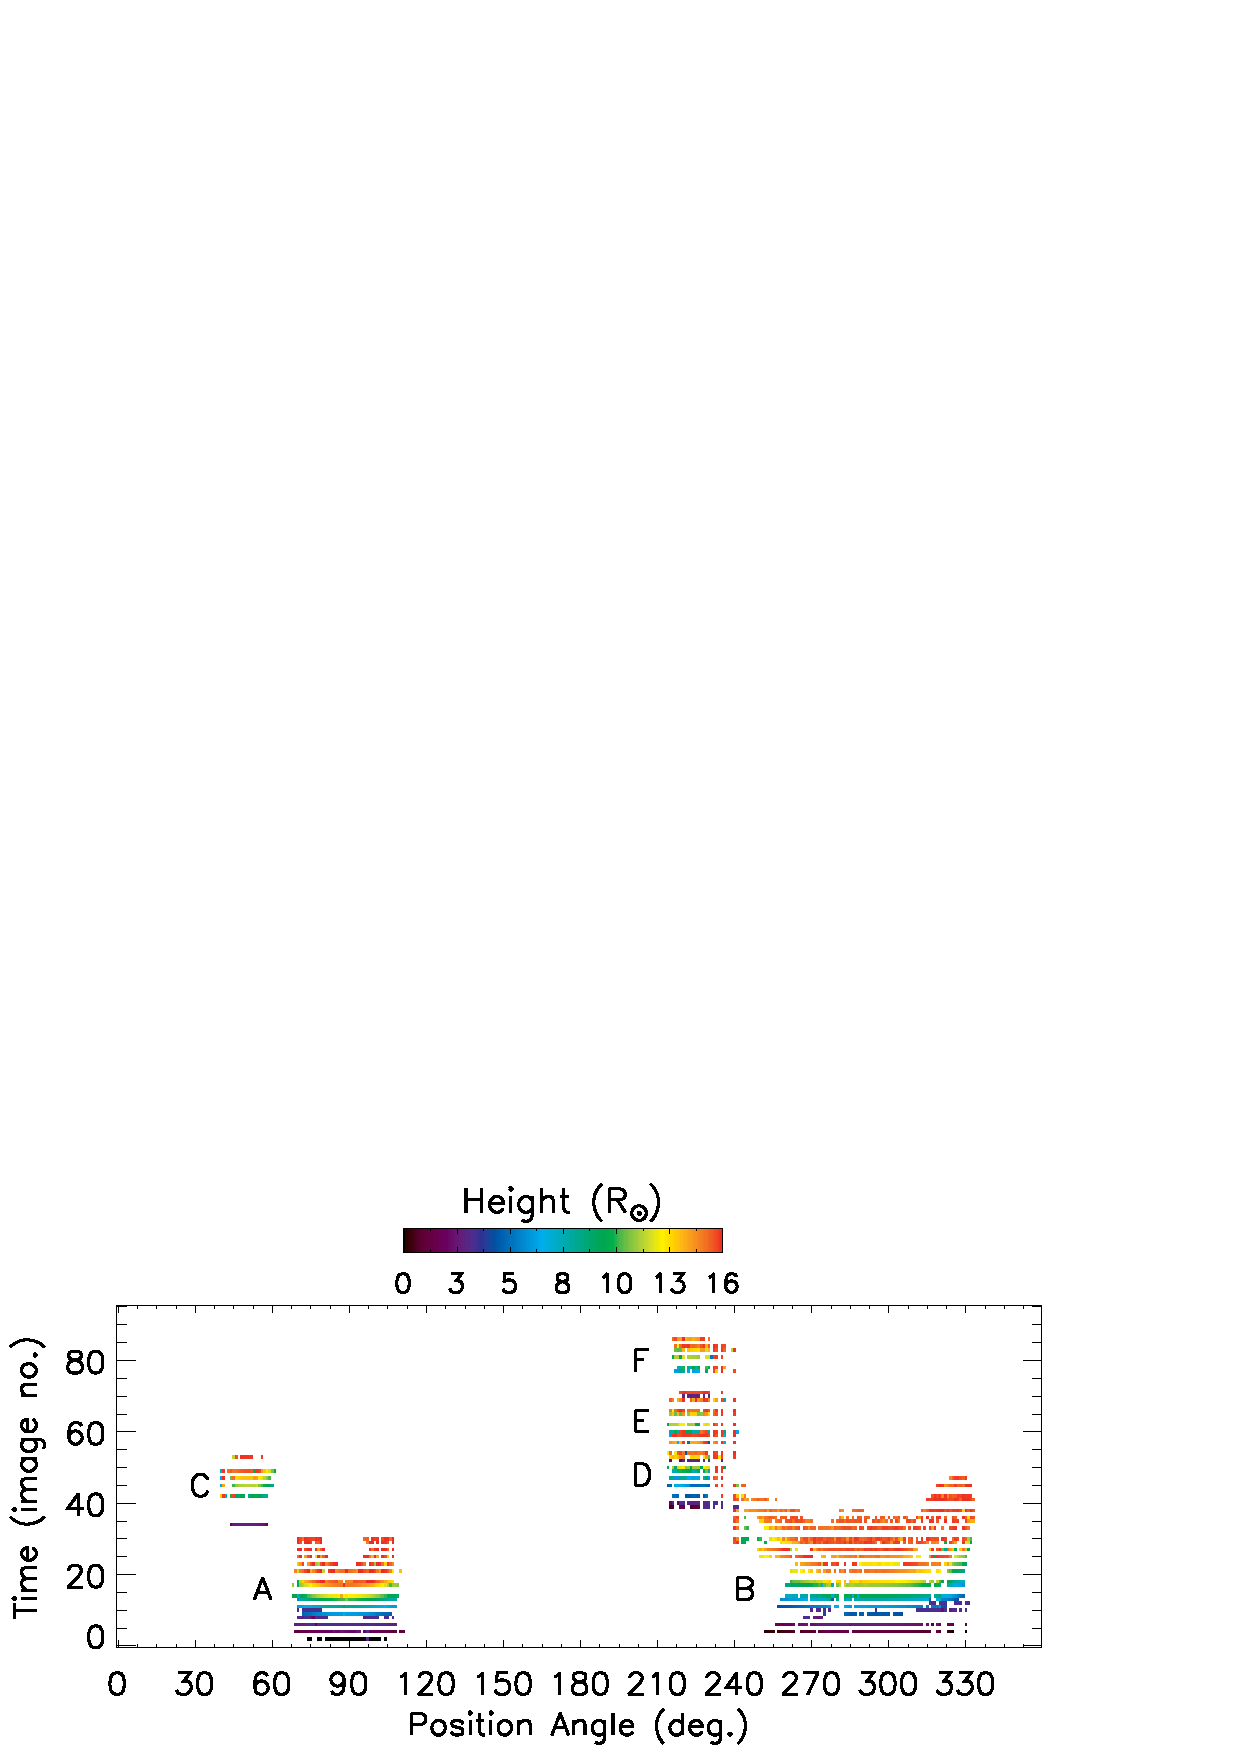
\includegraphics[scale=0.6, clip=true, trim=0 190 50 150]{images/figure_model_stack.pdf}}
\caption{The model CME detection stack, plotted in time, i.e., image number, against position angle measured counter-clockwise from solar north. The intensity corresponds to the height of the outermost points in the detection relative to sun-centre.}
\label{figure_model_stack}
\end{figure}

As the detections are performed through time, the information from them may be collated into a 3D stack of `Image Number' versus `Position Angle' versus `Height' (from sun-centre). For the purposes of determining the kinematics of CMEs, the outermost points along the detected CME structure are recorded as the CME height, measured along radial lines drawn  at 1$^{\circ}$ intervals across the plane-of-sky from sun-centre, with position angle taken counter-clockwise from solar north. A CME detected at a particular span of position angles through a sequence of frames will appear as a block of variable intensity in the 3D stack. An example of this is shown  in Figure~\ref{figure_model_stack} for a run of six model CMEs: three flux rope events, A, B, and C, launched at position angles 90$^{\circ}$, 290$^{\circ}$, and 50$^{\circ}$ respectively; and three plasma blobs, D, E, and F, in direct sucession of each other at position angle 225$^{\circ}$. The relative increase in intensity through the detection stack is indicative of the increasing CME height as it propagates out through the corona. Similarly, the angular span of the detections is indicative of the angular width of the CME. Trailing material contained within the internal structure of the CME will also be apparent on the detection stack as the CME front moves out of the field-of-view. Any residual streamer flows that are detected will also appear in the detection stack. However, they should only span small angular widths, and should not change much in their intensity since they do not undergo significant changes in height (being relatively static compared to the CMEs).

Upon inspection of the detection stack, the areas corresponding to CMEs (as opposed to streamer detections or noise) may be automatically isolated by the following criteria:
\begin{enumerate}
\item detections that lie within two time steps of each other are grouped;
\item detections that span $<$\,7$^{\circ}$ and do not have adjoining detections within 7$^{\circ}$ are discarded;
\item remaining detections that have not been grouped with at least two other detections are discarded.
\end{enumerate}
The resulting detection stack provides a cleaner output for determining the CME kinematics and morphology. The height information at each position angle of the isolated detection groups may be recorded and used to derive velocity and acceleration information across the angular span of the CME. Changes to its angular width may also be recorded as an indicator of its expansion. Thus a final output of information on each CME detection can include CME height, velocity, acceleration, observation time, position angle, trajectory, and angular width.

Figure~\ref{figure_proposal_events} shows the automatic CME detection and tracking algorithms applied to four real-data CME events following  processing with the NRGF (section~\ref{sect_nrgf}) and quiescent background separation technique (section~\ref{sect_separation}). The figure shows the LASCO/C2 and C3 CME detections, and resulting height-time profiles, for events that occurred on 01-Jan-00, 18-Apr-00, 23-Apr-00, and 13-Jan-11. The LASCO CME images show a snapshot of the CMEs' propagation through the C2 and C3 fields-of-view, with the automatic structure detection overlaid in yellow, and the outermost points along the the CME front highlighted in red. The height-time profiles show the CME heights measured in the radial direction corresponding to position angles counter-clockwise from solar north. The height-time profiles convey the different speeds attained along the expanding CME front, and can reveal strong initial acceleration (e.g., 18-Apr-00) or deceleration (e.g., 23-Apr-00).

It is further apparent how the detailed structure of the CMEs is highlighted through these methods of automated detection. The chosen multiscale filters lend themselves to the use of a pixel-chaining algorithm that characterises the edges in the detected CMEs. This essentially traces out the underlying magnetic field morphology of the CME event. This is of huge benefit to the field of solar physics where traditional image processing techniques (namely running or fixed differencing) introduce spatio-temporal crosstalk to the images and thus contaminate the true coronal structure. The fact that the detections are performed on single images also means the uncertainty in the time-dimension is on the order of the exposure time of the instrument rather than booming through differencing techniques, and this along with the precision of the multiscale filtering provides a high degree of accuracy in the final results.

\begin{figure}[!p*]
\centerline{\includegraphics[scale=1.2, clip=true, trim=0 340 180 10]{images/figure_proposal_events.pdf}}
\caption{A snapshot of the algorithms applied to the model CMEs A and B. Panels ($a$) and ($b$) show the magnitude information (edge strength), and ($c$) and ($d$) show the angular information, at a particular scale of the multiscale decomposition. Panels ($e$) and ($f$) show the resulting CME detection masks following the scoring system. Panels ($g$) and ($h$) show the final CME structure detection overlaid in yellow on the model C2 and C3 images. The edges were determined using a pixel-chaining algorithm on the magnitude and angular information of the multiscale decomposition.}
\label{figure_proposal_events}
\end{figure}





%%% %%%%%%%%%%%%%%%%%%%%%%%%%%%%%%%%%%%%%%%%%%%%%%%%%%%%%%%%%%%
%% Bibliography
%
% Using BibTeX
%
 \bibliographystyle{spr-mp-sola.bst}
% %\bibliographystyle{spr-mp-sola-cnd} %% Alternative style: no title, no concluding page
 \bibliography{references.bib}  
%
% Without BibTeX 
% \begin{thebibliography}{}
% \bibitem[\protect\citeauthoryear{Author}{Year}]{key}
%   <bibliographical entry>
%
% \bibitem[\protect\citeauthoryear{}{}]{}
%   
%  
% \end{thebibliography}

\end{article} 
\end{document}
